%=====================================================================
%  MCAIT 2026 - Track 2 (Applied and Domain-Specific AI)
%  CAMERA-READY MANUSCRIPT (de-anonymised)
%
%  Compile: pdfLaTeX, twice. No BibTeX (inline thebibliography).
%  Needs fig1_arch.png, fig2_bound.png, fig3_block.png alongside this file.
%  IEEEtran defaults to US Letter, which EDAS accepts.
%
%  ANONYMITY SWITCH: change \sys to "the proposed system" for a stricter
%  double-blind reading. Nothing else needs to change.
%=====================================================================
\documentclass[conference]{IEEEtran}
\IEEEoverridecommandlockouts

\usepackage{cite}
\usepackage{amsmath,amssymb}
\usepackage{graphicx}
\usepackage{textcomp}
\usepackage{booktabs}
\newcommand{\tbd}[1]{\textbf{[TBD: #1]}}
\newcommand{\sys}{Arcana}
\newcommand{\tbl}{\footnotesize}

\begin{document}

\title{Graph-Grounded Generative User Interfaces\\ for Learning: Retrieval Structure Determines\\ Interface Expressiveness}

\author{\IEEEauthorblockN{Fakhrul Azim Bin Ahmed Mardzukie}
\IEEEauthorblockA{Department of Computer and Information Sciences\\
Universiti Teknologi PETRONAS, Seri Iskandar, Perak, Malaysia\\
fakhrul\_22012087@utp.edu.my}}

\maketitle

\begin{abstract}
A learner working across their own documents is given a chat box and a stream of prose, because conventional retrieval augmented generation scores each passage independently and holds no representation of how sources relate. Systems can now generate interfaces on demand, but from model output rather than retrieved evidence, and in education an attractive presentation of an unsupported claim implants misconceptions that are hard to undo. This paper reports a learning workspace in which the interface answering a question is composed at request time: documents are extracted into a knowledge graph alongside a vector index, retrieval fuses graph traversal with dense and sparse signals by rank, and the model emits typed component selections carrying payloads built from retrieved evidence, each validated against a shared schema and rejected on any violation. The two layers are not independent: a component is a claim about the shape of an answer, so a comparison grid or contradiction alert cannot be honestly filled from passages ranked in isolation; retrieval structure bounds which components an interface can offer. We state the bound formally, give a pre-registered evaluation protocol with an ablation harness and an extraction-quality audit, and report a pilot run whose null result locates the current ceiling on the graph signal in query entity resolution. No claim about learning outcomes is made.
\end{abstract}

\begin{IEEEkeywords}
generative user interfaces, knowledge graphs, retrieval-augmented generation, adaptive learning, educational technology, learning interfaces
\end{IEEEkeywords}

%=====================================================================
\section{Introduction}
%=====================================================================

Retrieval augmented generation grounds a language model in material it was never trained on, retrieving passages at query time and conditioning its answer on them, which is what lets a learner question their own lecture notes and texts \cite{ref:gao}; fusing dense similarity with sparse keyword matching is an established gain over either alone \cite{ref:hybridrag}.

That architecture carries a limitation which never produces a visible error. In a flat retriever every chunk is scored independently of every other, so the system reliably finds the passage most similar to a question and has no representation for the facts that two passages disagree, that one concept is a prerequisite for another, or that an answer is distributed across documents none of which contains it alone. Embedding similarity encodes how alike two pieces of text are, not how the entities inside them connect. This is not a tuning problem a larger embedding model resolves, and it is not a prompt problem. Graph based retrieval addresses it by changing what is stored, extracting entities and relationships into an explicit graph and answering partly by traversal \cite{ref:edge}.

The consequence is usually discussed in terms of answer quality. We argue it is also, and more visibly, a consequence for the interface. The questions that advance a learner's understanding across many papers are relational: which agree, where they conflict, what the set does not cover, how an argument in one depends on a definition in another. A flat system can answer only with prose that asserts relations it never retrieved, handing the synthesis back as more text to read, which is the opposite of what a learner short on time and working memory needs \cite{ref:mayer}. Comparison grids, concept maps, and contradiction views are ordinary artifacts of study, and interactive representations can substantially outperform traditional instruction, with a pooled effect of $d = 0.83$ across twenty physics studies \cite{ref:phetmeta}. They are absent from corpus tools because building one requires that someone authored it for that topic in advance, and because the retrieval layer has nothing structured to fill it with.

Generative user interfaces remove the first obstacle, producing custom interfaces for arbitrary requests that are preferred to plain text in the large majority of comparisons and rated comparable to expert crafted work in roughly half \cite{ref:leviathan}. In education the capability has been applied at authoring time, in courseware generation \cite{ref:maicui}, tutor authoring \cite{ref:calo}, and adaptive support around existing content \cite{ref:learnmate}, with a reviewing human between generation and learner. That is what makes these systems safe, and what bounds them to what an educator anticipated.

Removing that human raises an objection the field has already stated: runtime generative interfaces are unsafe because verification cannot be conducted at scale \cite{ref:neshaei}. The caution is well founded. Factual error in instruction corrupts concepts that are hard to unlearn \cite{ref:eduevaldb}, learners detect errors in output they can execute but not in conceptual content \cite{ref:shoufan}, and surface plausibility is no check: of 43,677 generated programs passing public tests, 23,081 still failed hidden ones \cite{ref:codemonitor}.

Our position is that the objection is decisive against generating the interface from the model's own output, not against the idea itself. If the model is confined to choosing among existing components and filling them with retrieved evidence, what a learner sees is bounded by what the corpus supports. The retrieval layer then becomes load bearing, and the interface layer needs the discipline developed for generated artifacts elsewhere: a contract, a check before delivery, and a delivery path that cannot carry output which failed it.

This paper reports \sys{}, a learning workspace built on that principle. Its contributions are:

\begin{enumerate}
\item An architecture coupling graph native hybrid retrieval to a typed generative interface, in which entities and relations extracted at ingestion are fused with dense and sparse retrieval by rank, and the resulting evidence populates interface components rather than prose (Section~\ref{sec:method}).
\item A generative interface composed at request time rather than authored per topic, held to the standard developed for verified generated artifacts: one schema generating both sides of the wire, validation that fails closed, registry-only rendering, and provenance on every rendered claim, so that a malformed or unregistered presentation is not representable (Section~\ref{sec:genui}).
\item A formal statement, with a component by component mapping to study activities, that retrieval structure bounds interface expressiveness (Section~\ref{sec:bound}).
\item An evaluation protocol committed before any run, comprising an ablation harness separating the dense, sparse, and graph signals, a paired test of graph-hybrid against flat retrieval, and an extraction-quality audit procedure, together with a pilot run whose result is reported as found (Section~\ref{sec:results}). We mark which claims are architectural, which are measured, and which remain unmeasured.
\end{enumerate}

%=====================================================================
\section{Related Work}
%=====================================================================

\subsection{Retrieval, and its flat ceiling}
Surveys trace a progression from naive retrieve-then-generate through modular pipelines, with retrieval consistently the weakest stage \cite{ref:gao}, and hybrid retrieval fusing dense and sparse signals is a documented improvement over either alone \cite{ref:hybridrag}. Both signals rank passages independently, so every improvement in this family changes which passages return, not what can be said about how they connect. Graph based retrieval changes what is stored, extracting entities and relationships and answering partly by traversal \cite{ref:edge}, a space since organised into graph indexing, graph guided retrieval, and graph enhanced generation \cite{ref:han}, with systems reaching competitive accuracy through personalised centrality over a schema free graph \cite{ref:hipporag} or dual level retrieval at a fraction of the token cost \cite{ref:lightrag}. Schema free extraction removes the need for a predefined ontology \cite{ref:edc}, which matters when a learner's documents may come from any discipline. \emph{The gap:} this literature evaluates graph retrieval \emph{as retrieval}, scored by answer quality, and extraction as extraction; neither treats retrieved structure as a substrate for presentation, which is the connection this paper draws.

\subsection{Generative user interfaces}
Current work establishes feasibility, showing generated interfaces are robustly producible for arbitrary prompts and preferred to markdown output \cite{ref:leviathan}, and then alignment, tuning them to user preference from crowdsourced data \cite{ref:alignui,ref:crowdgenui}. A parallel line specifies declarative protocols for streaming typed interface intent to a trusted component registry rather than shipping markup \cite{ref:a2ui}. \emph{The gap:} these systems are evaluated for preference and perceived quality. None asks whether the content presented is supported by a source, and preference is not a proxy for correctness in instruction.

\subsection{Generated artifacts in education}
Educational applications keep a human in the loop: generative components in tutor authoring environments for non-technical educators \cite{ref:calo}, courseware generated from textbooks through a generate, verify, and optimise pipeline with classroom evidence \cite{ref:maicui}, and adaptive systems coordinating support around fixed material \cite{ref:learnmate}. Prompt templates yield interactive physics simulations only after iterative human debugging \cite{ref:promptsim}, and an immersive chemistry system achieves safety by restricting output to a rigid specification rendered by a fixed renderer, capping expressiveness in exchange \cite{ref:chemersive}. \emph{The gap:} all are authoring time and educator facing, or achieve safety by schema restriction alone. None generates for the learner at request time from retrieved evidence, and the position that runtime generation cannot be made safe \cite{ref:neshaei} stands without a mechanism that would refute it.

\subsection{Verification, and the risk of generated instruction}
Adversarial verification is well developed for code, hardening specifications with counter-implementations \cite{ref:probe}, naming pseudo-correctness as the failure mode \cite{ref:advermcts}, and scaling by decomposing criteria \cite{ref:kwok}. These verify against oracles and executable contracts; an educational presentation has neither, so what transfers is the discipline rather than the technique. On the learning side, multimedia learning theory explains why representation choice matters \cite{ref:mayer}, while generated instruction carries specific risks of concept corruption \cite{ref:eduevaldb} and a verifiability gap for learners \cite{ref:shoufan}. \emph{The gap:} adaptive learning personalises the sequence of material that already exists; it does not generate the presentation, and so never confronts what a generated presentation is permitted to assert.
%=====================================================================
\section{Methodology: System Design}
\label{sec:method}
%=====================================================================

\subsection{Overview}
The work follows a design and evaluation methodology: the architecture is specified and implemented (this section and Section~\ref{sec:genui}), its central property is stated formally and argued from component preconditions (Section~\ref{sec:bound}), and its empirical claim is tested against a protocol committed before any run (Section~\ref{sec:results}). \sys{} is a workspace for a learner working across their own corpus of lecture material, papers, and notes. A question returns not a paragraph but a set of interface components, such as a cited summary, a comparison grid, a contradiction alert, or recall cards. The components are fixed; what is generated per request is which components the answer requires and the evidence that fills them (Fig.~\ref{fig:arch}).

\begin{figure}[t]
\centering
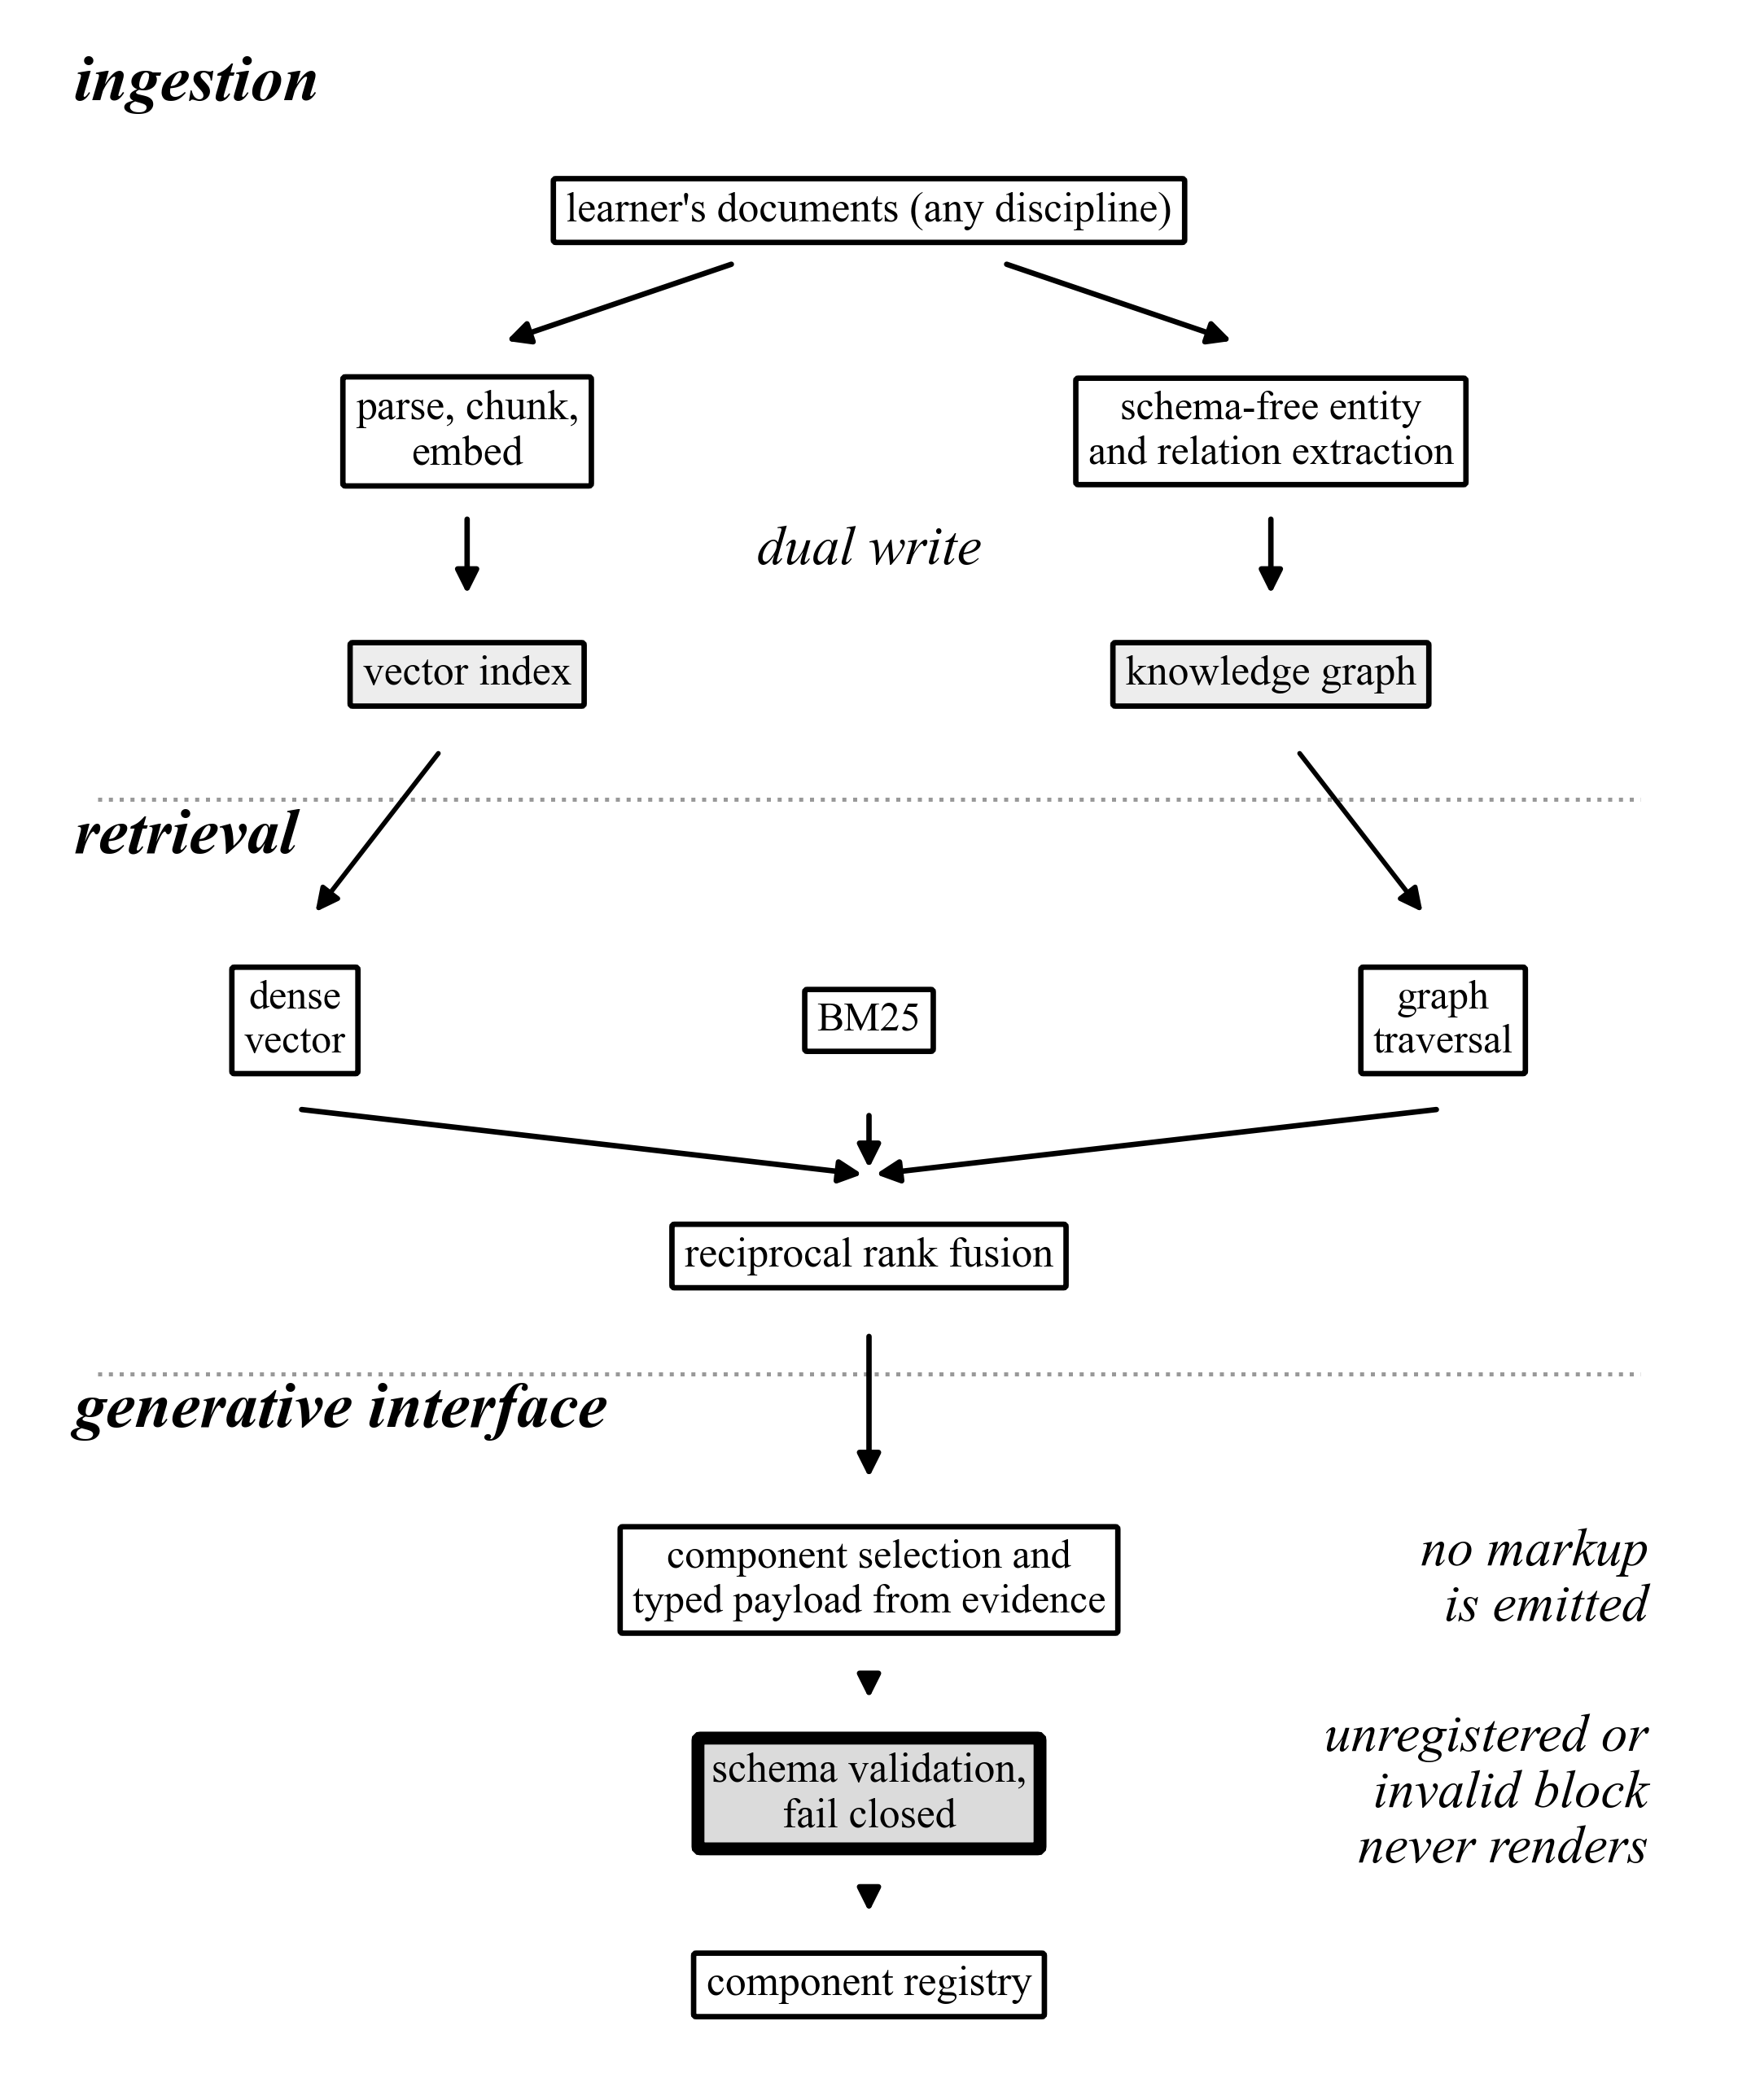
\includegraphics[width=\columnwidth]{fig1_arch.png}
\caption{From document to rendered component. Ingestion writes the vector index and graph in one pass, retrieval fuses three signals by rank, and fail-closed validation sits between component selection and the registry.}
\label{fig:arch}
\end{figure}

\subsection{Ingestion and graph construction}
An ingested document is parsed, chunked, and embedded, and in the same pass entities and relationships are extracted without a predefined ontology, following the extract, define, and canonicalise pattern \cite{ref:edc}; schema freedom is a requirement, since a learner's corpus may span any discipline. Output is written to the vector index and the graph in one pass, so retrieval queries two representations of the same material rather than two divergent corpora.
\subsection{Hybrid retrieval}
At query time three signals are computed. Dense vector similarity returns passages semantically close to the question. Sparse keyword matching returns passages sharing its terms, recovering exact identifiers and rare terms that embeddings blur. Graph traversal expands from entities the question resolves to, scoring chunks in which those entities and their one-hop neighbours are mentioned. The three ranked lists are combined by reciprocal rank fusion \cite{ref:rrf}: for a document $d$ retrieved by a set of rankers $R$, where $r(d)$ is its rank from ranker $r$ and $k$ is a smoothing constant,

\begin{equation}
\mathrm{RRF}(d) = \sum_{r \in R} \frac{1}{k + r(d)}.
\end{equation}

Fusing by rank is what makes the combination possible at all, since cosine similarity, keyword relevance, and traversal scores are not comparable quantities. The vector and keyword pair is established as superior to either alone \cite{ref:hybridrag}; graph traversal is the signal under test in Section~\ref{sec:results}.

\subsection{Orchestration and personalisation, in brief}
Between retrieval and presentation sits a layer of task specialised agents on a graph orchestration framework \cite{ref:langgraph}, following the role specialisation established for collaborative agent frameworks \cite{ref:metagpt}, so that comparison, contradiction detection, study artifact generation, and written work can use different tools and retrieval patterns. Two properties of that layer matter here. Agents never import one another: every hand-off passes through a single routing function within hop and token budgets, so the topology is auditable at one boundary rather than distributed across call sites, a deployable answer to the observation that static orchestration graphs fix their topology at design time \cite{ref:adaptorch}. And every request path terminates at the component selection stage of Section~\ref{sec:genui}, so no agent can return to the learner directly, which is what makes the interface guarantees enforceable rather than conventional.

Trained personalisation models, for re-ranking and review scheduling, are specified and not trained; they are strictly additive, and no claim in this paper depends on them.
%=====================================================================
\section{The Generative Interface Layer}
\label{sec:genui}

\subsection{Generation at request time}
Nothing in this system is authored per topic. When a learner asks a question, the interface answering it is assembled at that moment: which components appear, in what order, filled with what, and in which layout. A differently shaped question about the same corpus receives a differently shaped interface, and neither existed until it was asked for. Authoring time systems generate \emph{beforehand}, so their coverage is the set of questions an educator anticipated; removing the authoring step changes coverage from enumerable to open.

The move that makes it safe is to relocate where the generative freedom sits. The model does not write the interface, it composes one. Its output is a sequence of typed component selections, each with a payload conforming to that component's schema and built from retrieved evidence; layout, typography, and interaction are implemented in the component and are not under model control. With a catalogue of $n$ components and an ordered selection of $k$ of them, each with a payload whose structure is derived per query, the space of expressible interfaces is combinatorial in $n$ and $k$ and unbounded in payload structure. A comparison grid is one component; its dimensions, rows, and cells are decided per question from what the graph holds. Nobody authored the columns.

Table~\ref{tab:regimes} places the three regimes against one another. Authoring time systems are safe and bounded by anticipation. Markup emitting runtime systems are unbounded and, by the field's own assessment, unverifiable at scale \cite{ref:neshaei}. Composing at request time from a verified vocabulary takes the coverage of the second and the accountability of the first, and pays for it in the ceiling discussed in Section~\ref{sec:limits}.
\begin{table}[t]
\caption{Three regimes for producing a learning interface}
\label{tab:regimes}
\centering
\tbl
\begin{tabular}{@{}p{0.22\columnwidth}p{0.20\columnwidth}p{0.20\columnwidth}p{0.22\columnwidth}@{}}
\toprule
& \textbf{Authored ahead} & \textbf{Markup emitted at runtime} & \textbf{Composed at request time} \\
\midrule
Coverage & what was anticipated & any question & any question \\
Produced by & a person & the model, as code & the model, as typed selections \\
Correctness rests on & human review & post-hoc verification & retrieved evidence and schema \\
Expressiveness & fixed catalogue & unbounded & combinatorial over a vocabulary \\
Failure mode & no answer exists & confident wrong artifact & closest available component \\
\bottomrule
\end{tabular}
\end{table}

\subsection{A worked request}
\label{sec:worked}
Consider a learner revising chemistry from a corpus of their own lecture notes, a textbook chapter, and worked solutions. They ask why raising the temperature increases the rate of a reaction.

The notes attribute the increase to particles colliding more often; the chapter attributes it principally to a larger proportion of collisions exceeding the activation energy. Both mechanisms are real, and the difference in emphasis is what a learner reproduces in an examination answer without noticing. A flat retriever ranks each passage on its own similarity, so whether both surface together is incidental. The graph links them through a shared entity across document boundaries, so they arrive in the same retrieved set, which is the precondition for a component that does the reconciliation visibly; Section~\ref{sec:contra} states what the system then does with it.

The response composes three blocks: a cited summary with citations to both sources; a contradiction alert presenting the two attributions side by side, each with its source; and a concept map connecting temperature to collision frequency, the activation energy threshold, and the fraction of effective collisions. None was authored for this question, and the alert could not have been, since the divergence exists only between this learner's notes and this chapter. Nothing in the path is chemistry specific. A biology question spanning the nervous and endocrine systems yields a comparison grid instead; the vocabulary is the same, and the composition and evidence are not.

Table~\ref{tab:payload} gives the alert's payload exactly as the shipped schema declares it, with what each field is grounded in and what produces it. Every field is populated from retrieved passages, and the right-hand column shows where the pipeline enforces that and where it currently rests on the detection pass.
\begin{table}[t]
\caption{Payload of one component as declared in the shared schema, with the grounding and the producer of each field}
\label{tab:payload}
\centering
\tbl
\begin{tabular}{@{}p{0.19\columnwidth}p{0.15\columnwidth}p{0.26\columnwidth}p{0.22\columnwidth}@{}}
\toprule
\textbf{Field} & \textbf{Type} & \textbf{Grounded in} & \textbf{Produced by} \\
\midrule
concept & string & the entity the claims address & detection pass, falling back to the query \\
summary & string & the retrieved passage set & detection pass over retrieved chunks only \\
claims & list & one retrieved passage each & detection pass, defensively parsed \\
claim.docId & document ref & a document in the learner's corpus & detection pass, from ids supplied with each passage \\
claim.docTitle & string & the cited document & detection pass \\
claim.stance & string & the position that document takes & detection pass over the passage \\
claim.quote & string & a span of its source passage, capped at 200 characters & detection pass; verbatim match specified, not yet enforced \\
meta.panel & enum & the workspace region & composition stage \\
meta.order & number & position among sibling blocks & composition stage \\
meta.status & enum & one of the four render states & streaming stage \\
\bottomrule
\end{tabular}
\end{table}

\subsection{How a contradiction is computed}
\label{sec:contra}
Because a contradiction alert is the strongest claim the catalogue makes, its derivation is stated in full. Given a query $q$, the agent retrieves $E(q)$ by the fused path at depth 10, and returns no block when $E(q)$ is empty. A single versioned prompt, which presents each passage with its document id, identifies within $E(q)$ positions attributed to different documents on one concept. The response is parsed defensively into at most four typed claims; malformed claims are discarded rather than repaired, and an unparseable response yields an alert with no claims. Each claim carries a document id, title, stance, and a quotation capped at 200 characters, all taken from this detection pass. The pipeline does not yet check that a quotation appears verbatim in a retrieved chunk of the document it names; that check is specified, and its absence is a limitation (Section~\ref{sec:limits}). The block is then validated and streamed.

Two consequences are limitations as much as design decisions. The relation is detected over the retrieved set by a language model rather than read off a typed edge, so the graph's contribution is to place mutually relevant passages from different documents into $E(q)$, not to assert the disagreement itself. And the payload carries no numeric confidence: a calibrated confidence is specified but not computed in the running system, so the schema declares no field the system cannot honestly fill. A confidence the model assigned to its own output would be exactly the self-report this architecture exists to avoid.

\subsection{The wire contract, validation, and the registry}
Every object crossing from server to client is a typed block carrying a discriminating type tag, a payload whose shape is fixed by that tag, and metadata giving panel, order, and render state. Nothing else crosses the wire, and there is no escape hatch for free text. Provenance is carried inside the payload, as citation identifiers and as a document id with a quotation on each claim. Block and payload types are defined once in a shared schema package, and server side model classes are generated from it, so a payload change not reflected on both sides is a compile error rather than the silent producer and consumer drift common in streaming interface protocols. Adding a component is a three step change: add the schema variant and regenerate, implement the component with its four states, and add one line to the registry. Any change that instead touches the streaming layer, the validator, or the selection logic is off pattern by construction.

Every block passes a validator on the server before it is streamed. The validator dispatches on the type tag through a discriminated union, re-validates model instances rather than trusting them, so a payload mutated after construction cannot ride through on the strength of its type, and turns any violation into a structured error envelope carrying the offending field paths rather than a partial render. Validation runs on the server rather than the client, where a failure would arrive after the learner is already looking at the region it was meant to fill. The direction of failure is the design decision. A validator that passes questionable payloads through in the hope the client copes will, in an educational setting, render something the learner reads as authoritative; failing closed converts a data defect into a visible error state, which is recoverable, rather than a confident wrong presentation, which is not, the reasoning that leads verification work in code generation to reject rather than repair \cite{ref:probe}.

The client maps a type tag to a component through exactly one registry, enforced at type level, so an unregistered block has no path to the screen and omitting registration fails the build. Each component implements four states: \emph{empty}, which must read as an answered question; \emph{loading}; \emph{partial}, for a payload arriving progressively; and \emph{error}, with a retry affordance. Blocks stream over server sent events as they are produced, so a learner sees the answer assemble: the cited summary appears while the contradiction alert is still being built. \emph{Partial} is therefore the normal condition of a composed interface in flight, not an error. The workspace itself reshapes with the task, because the components that serve surveying, revising, drafting, and Socratic questioning differ; mode is inferred from the request rather than set by a control the learner must find.

\subsection{Grounding and the standards this layer is held to}
No synthesis occurs without retrieved evidence in hand, and cited summaries pass a claim verification stage before their block is built. A fact-checking agent receives the summary and each citation's quotation, truncated at 280 characters, and in one call under a versioned prompt judges per citation whether the quotation contains explicit evidence for the claim it is attached to, with topical overlap alone not counting as support. This decomposes verification per claim rather than asking one global question about quality \cite{ref:kwok}. Citations judged unsupported are dropped when the interface agent builds the block, and the verdicts are recorded separately so they can be audited. Two limits are stated plainly: the judge is itself a language model whose accuracy is not yet measured, and if its call fails the citations are retained, so this stage fails open, unlike schema validation. The design still departs from preference aligned generative interfaces \cite{ref:alignui}: the check is not whether the presentation is good but whether each assertion is supported by a passage actually retrieved. Binding each block to the full ranked retrieval result that produced it is recorded in the audit log but not yet exposed through the API.

These standards derive from work on generated artifacts that must be correct before delivery, where a contract precedes the artifact, an adversarial check runs against it, and the delivery path cannot carry unchecked output \cite{ref:probe,ref:advermcts,ref:kwok}. Here the artifact is a typed block and the contract is the component schema, and each standard names the failure it contains: the shared schema stops drift, retrieval before synthesis restricts assertions to retrieved material, per-claim checking filters unsupported citations, failing closed stops malformed presentations, registry-only dispatch stops unregistered ones, and per-claim citation stops untraceable ones. An interface that misrepresents the corpus remains possible, as Section~\ref{sec:limits} states; one that is malformed or unregistered does not.
\section{Retrieval Structure Determines Interface Expressiveness}
\label{sec:bound}
%=====================================================================

Graph native retrieval and generative interfaces belong in one system because the second is bounded by the first, in a way that can be stated precisely. Since \emph{determines} is easily read more strongly than it is meant, we define it. Let $C$ be the component catalogue. For a component $c$ in $C$, let $P(c)$ be its \emph{structural precondition}, the relation its payload asserts among the evidence that fills it, and let $E(R, q)$ be the evidence a retrieval layer $R$ returns for a query $q$. Define the \emph{evidence-grounded relational expressiveness} of $R$ as the set of components whose precondition that layer can satisfy from retrieved evidence alone,
\begin{equation}
X(R) = \{\, c \in C \mid P(c) \text{ satisfiable from } E(R, q) \,\}.
\end{equation}
The claim of this section concerns $X$ and nothing else: $X(\text{flat})$ is a proper subset of $X(\text{graph-hybrid})$. It is not a claim that flat retrieval cannot render a comparison grid, since any renderer can draw one, but that filling it from a flat layer requires supplying from the model a relation retrieval never returned.

A typed component is a claim about the shape of an answer: a comparison grid claims documents align on shared dimensions, a contradiction alert that two statements address one entity and disagree, a concept map that concepts stand in labelled relations. If retrieval cannot supply that structure, filling the component means inventing it. Flat retrieval supplies ranked passages and sources, sufficient for a cited summary, a source list, and recall cards, and insufficient for every component whose meaning is a relation between passages (Fig.~\ref{fig:bound}).

\begin{figure}[t]
\centering
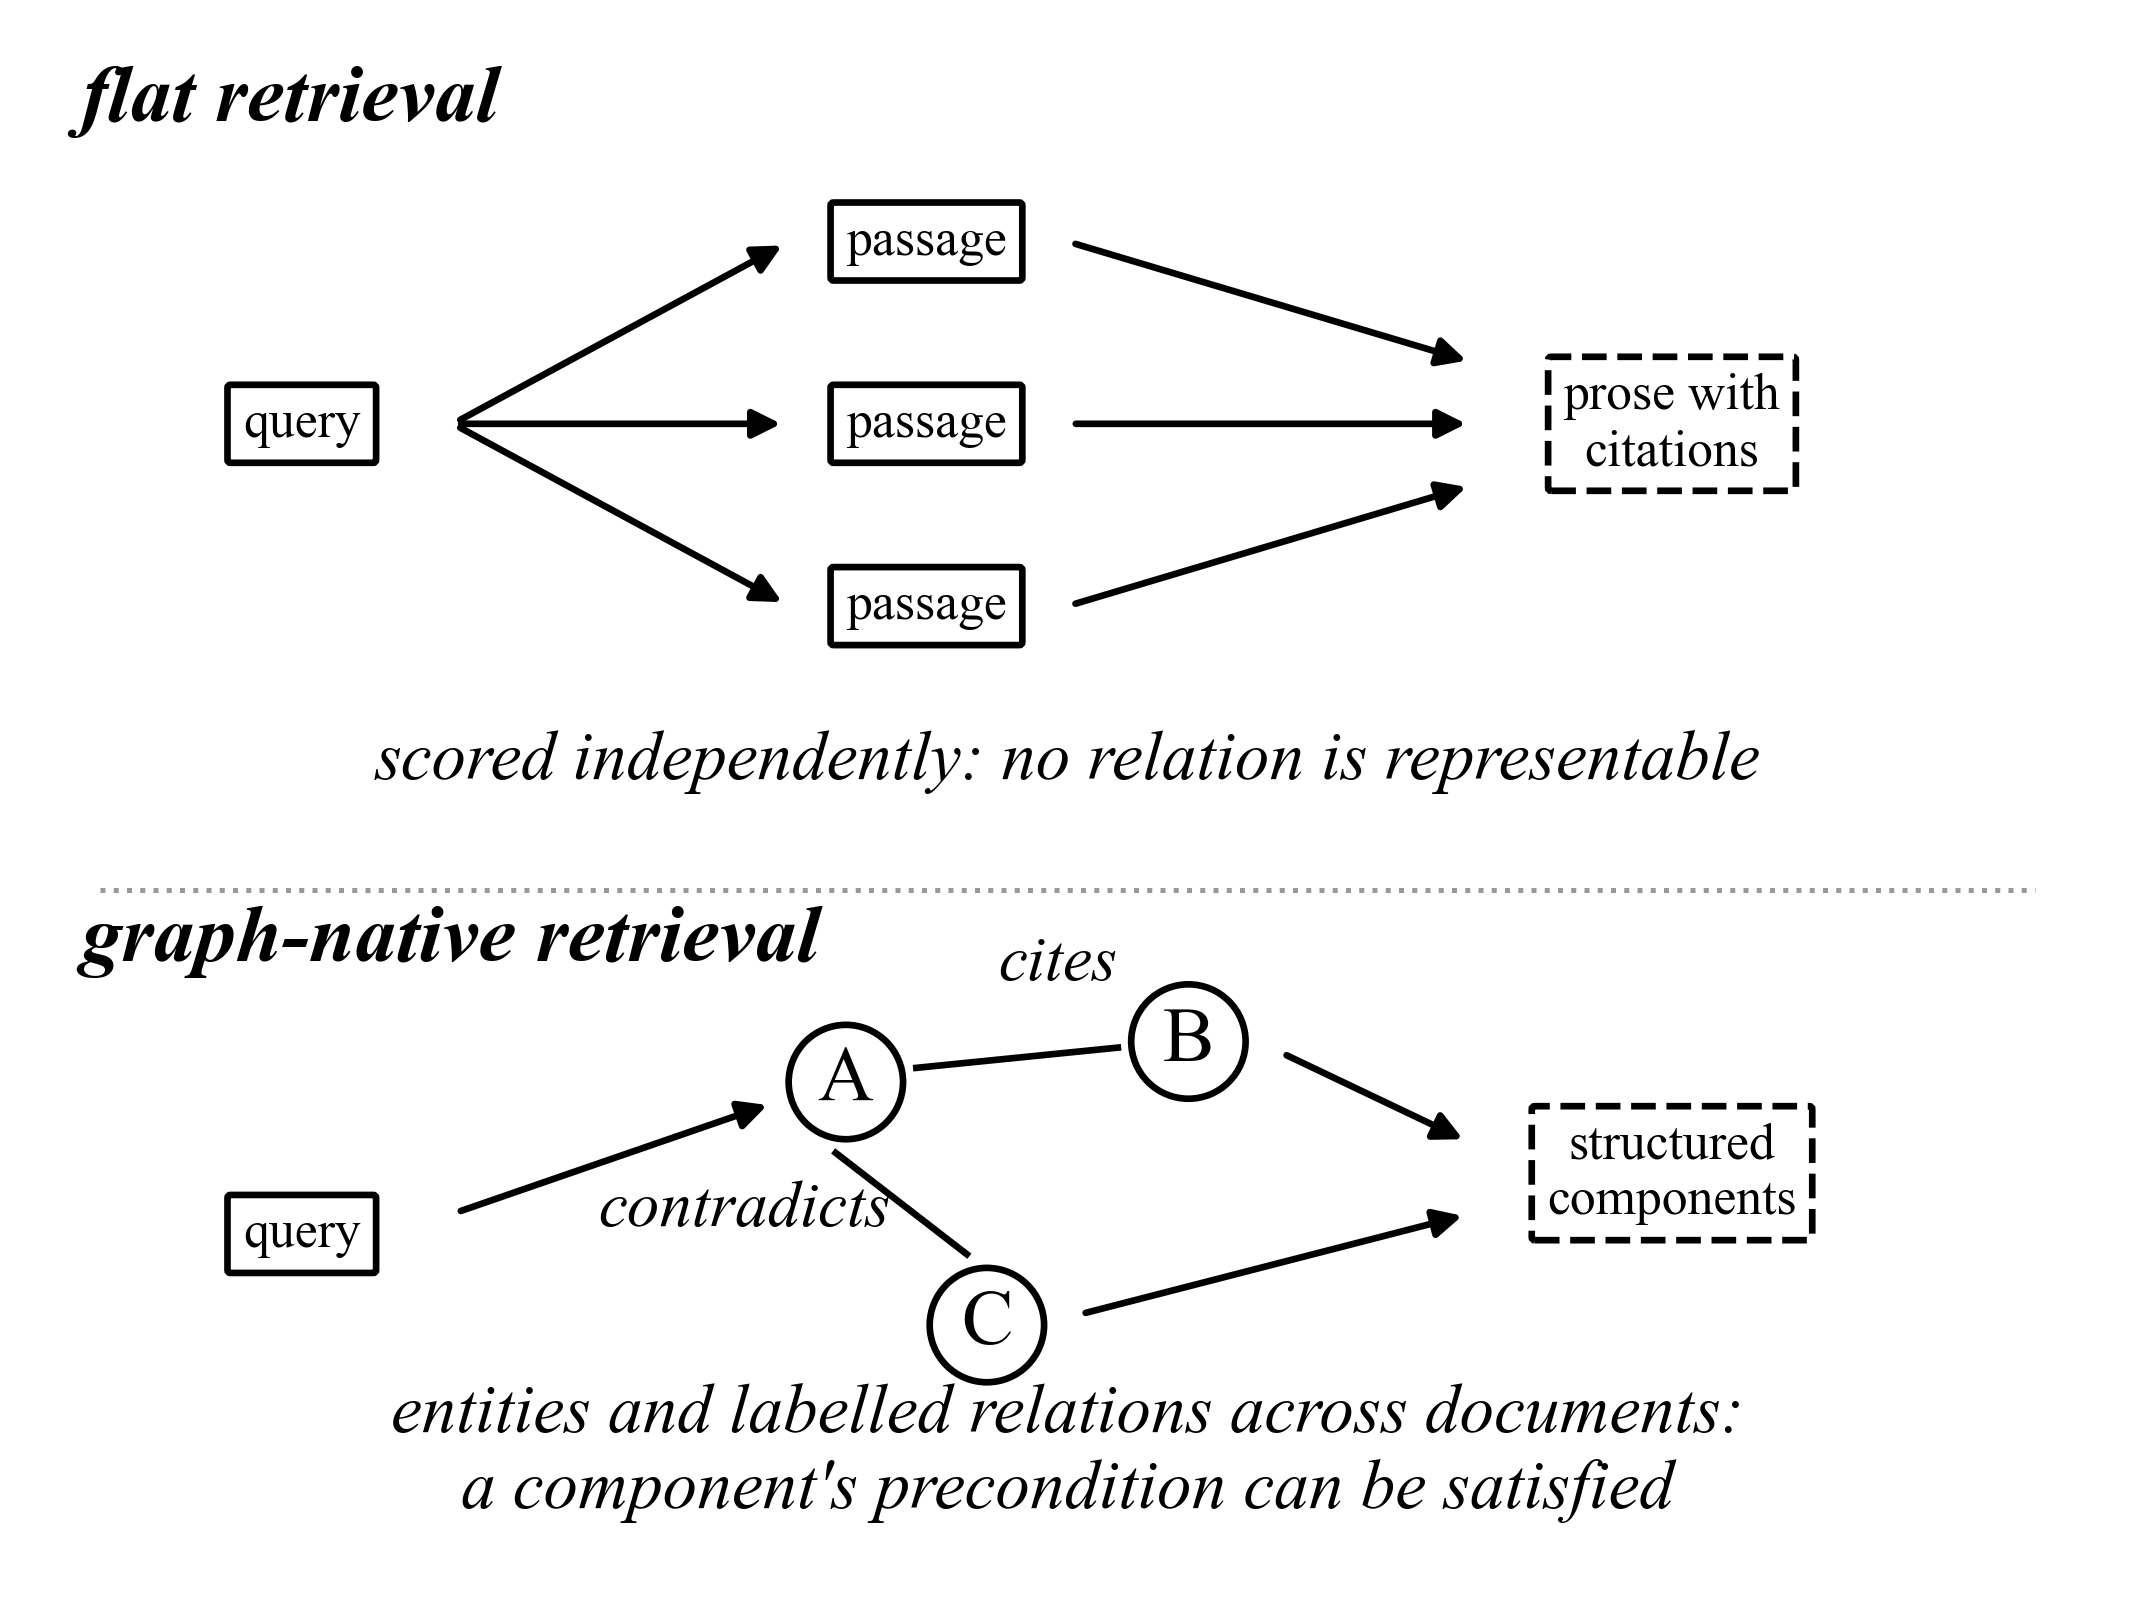
\includegraphics[width=\columnwidth]{fig2_bound.png}
\caption{Why retrieval bounds the interface. Independently scored passages justify cited prose; entities and labelled relations across documents are the precondition relational components assert.}
\label{fig:bound}
\end{figure}

Table~\ref{tab:bound} makes the mapping concrete and adds the study activity each component supports. The pattern is not incidental. Components flat retrieval can justify support reading and recall; components requiring graph structure support comparison, reconciliation, and finding what a corpus does not cover, the higher order activities a learner is least able to perform unaided and the ones associated with generative processing rather than passive intake \cite{ref:mayer}.

\begin{table}[t]
\caption{Component preconditions, the retrieval signal that supplies them, and the study activity each supports}
\label{tab:bound}
\centering
\tbl
\begin{tabular}{@{}p{0.19\columnwidth}p{0.28\columnwidth}p{0.19\columnwidth}p{0.19\columnwidth}@{}}
\toprule
\textbf{Component} & \textbf{Structural precondition} & \textbf{Supplied by} & \textbf{Study activity} \\
\midrule
Cited summary & ranked passages with sources & flat retrieval & reading, orientation \\
Source list & document metadata & document store & corpus review \\
Recall cards & atomic facts with sources & flat retrieval & retrieval practice \\
Comparison grid & two or more documents aligned on shared dimensions & cross-document entity alignment & comparison \\
Contradiction alert & claim pairs on one entity that disagree & cross-document co-retrieval via the graph & reconciling sources \\
Graph view & entities and labelled edges & the graph itself & structural overview \\
Concept map & concept-to-concept relations & graph traversal & organising knowledge \\
Timeline & events with temporal ordering & extracted temporal relations & sequencing \\
Gap analysis & coverage over a concept space & graph communities & finding blind spots \\
Insight card & a path between distant entities & multi-hop traversal & discovery \\
\bottomrule
\end{tabular}
\end{table}

The design rule that follows is this paper's practical claim: the catalogue a generative learning interface can honestly offer is a function of the retrieval layer beneath it. A system pairing flat retrieval with a rich catalogue is not richer; its extra components are filled by the model rather than by evidence, the failure the education literature warns about \cite{ref:eduevaldb,ref:neshaei}, in a more convincing package than prose.

We have removed the comparison with commercial corpus assistants that the submitted version carried: judging whether such a system grounds a structured component in retrieved structure needs documentation they do not publish or testing we have not run, and asserting it would be the unsupported claim this paper argues against.

%=====================================================================
\section{Results: Implementation Status and Evaluation}
\label{sec:results}
%=====================================================================

\subsection{What is established and what requires measurement}
Three claims in this paper are of different kinds and require different evidence. The interface guarantees are structural: that an unregistered or schema invalid block cannot reach the learner is a property of the wire contract and single point enforcement, established by construction and checked in continuous integration. The expressiveness bound is an argument from preconditions (Table~\ref{tab:bound}); measurement would add not whether it holds but what the components above the flat line are worth to a learner. The retrieval claim is empirical, and this section gives its protocol and a pilot run. No claim about learning outcomes is made anywhere in this paper.

\subsection{Protocol and setup}
\label{sec:setup}
\emph{Questions.} Twenty questions in three categories were committed to the project repository on 9 June 2026, before any benchmark execution, and are unchanged since: 12 cross-document questions, which require combining evidence from two or more sources and are where traversal is expected to help; 4 single-document controls, since a graph signal that helps its target cases while harming the rest is not an improvement; and 4 contradiction questions.

\emph{Corpus.} Sixteen retrieval and knowledge-graph papers from a public preprint server, listed by persistent identifier in a manifest fixed before any run, spanning 8 to 88 pages and yielding 1{,}570 chunks.

\emph{Arms and metrics.} Five arms: dense only, sparse only, graph only, flat (dense and sparse), and hybrid (all three), each the same pipeline with signals disabled, so only the active signals vary (Table~\ref{tab:settings}). Metrics are distinct source count, the direct proxy for the cross-document coverage the graph signal should add, and median latency; hybrid and flat are compared by a paired Wilcoxon signed-rank test. Citation recall needs gold annotation this study lacks, and model judged answer scores \cite{ref:ragas} would confound retrieval with generation.

\begin{table}[t]
\caption{Settings held constant across every arm}
\label{tab:settings}
\centering
\tbl
\begin{tabular}{@{}p{0.42\columnwidth}p{0.46\columnwidth}@{}}
\toprule
\textbf{Setting} & \textbf{Value} \\
\midrule
Chunk size, overlap & 1{,}200 characters, 200 \\
Embedding model & 3{,}072-dimensional, cosine \\
Sparse signal & BM25 over the same chunks \\
Graph construction & schema-free extraction, one pass per chunk \\
Fusion & reciprocal rank fusion, $k = 60$ \\
Depth & top 10 per signal and after fusion \\
Graph traversal & 1 hop from resolved query entities \\
\bottomrule
\end{tabular}
\end{table}

\subsection{Pilot run}
\label{sec:retrieval-results}
The full sixteen-document run has not been completed: entity extraction over the remaining corpus was interrupted by an exhausted model-provider quota, so no full-corpus result is reported. A pilot ran all 20 questions through all five arms with the vector index and graph built from 4 of the 16 documents (796 nodes, 859 edges). Table~\ref{tab:pilot} gives the result.

\begin{table}[t]
\caption{Pilot run: 20 questions, 4 of 16 documents indexed}
\label{tab:pilot}
\centering
\tbl
\begin{tabular}{@{}p{0.30\columnwidth}p{0.28\columnwidth}p{0.28\columnwidth}@{}}
\toprule
\textbf{Arm} & \textbf{Mean distinct sources} & \textbf{Median latency (ms)} \\
\midrule
Dense only & 2.50 & 670 \\
Sparse only & 3.35 & 208 \\
Graph only & 0.60 & 2{,}500 \\
Flat (dense + sparse) & 3.15 & 897 \\
Hybrid (all three) & 3.15 & 900 \\
\bottomrule
\end{tabular}
\end{table}

The result is null. Hybrid and flat tie on 18 of 20 questions, with one win and one loss (Wilcoxon $p = 1.0$), and differ by 0.08 sources on the cross-document category. The reason is visible in the graph-only arm: traversal returned no chunks at all for 15 of the 20 questions, so on those questions the hybrid arm was the flat arm. The pilot therefore does not test whether graph structure adds cross-document coverage; it shows that under this configuration the graph signal rarely fires.

The pilot ran under the original query entity resolution, which required an exact match to a graph node identifier. After the pilot that rule was replaced by approximate token matching, capped at three candidates and scored below an exact match, and a defect persisting the graph to a path the benchmark did not read was repaired. Both are declared as harness changes after registration; neither changes the question set.

\subsection{Knowledge-graph extraction quality}
\label{sec:extraction-quality}
A component grounded in a spurious edge is grounded in nothing, and an alert built on a mis-extracted relation looks exactly like a correct one. We therefore specify an audit procedure, implemented as a script in the evaluation harness. Edges are sampled at random under a fixed seed; the source passage for an edge is a chunk mentioning both endpoints, and an edge with none is unsupported. Each edge is judged supported, unsupported, or unclear against its passage, with a relation true in general but absent from the passage counted as unsupported; precision is reported with a Wilson interval and every judgement is kept as a per-edge record. The audit has not yet been run, since it is defined over the full graph. With a single automated annotator adjudicated by the author, no inter-annotator agreement will be reported; the per-edge records make the judgements auditable instead.

\subsection{Implementation status}
Table~\ref{tab:status} reports status verified against the running system rather than against the plan. Each row rests on an artifact in the public project repository (github.com/Azimlearning/Arcana): registry completeness is a build-time type check, validation and retrieval are covered by a test suite of 645 tests, all passing at camera-ready and run in continuous integration, and the pre-registered question set, corpus manifest, ablation and audit scripts, and the pilot's per-question results are released there.

\begin{table}[t]
\caption{Implementation status, verified against the running system}
\label{tab:status}
\centering
\tbl
\begin{tabular}{@{}p{0.53\columnwidth}p{0.35\columnwidth}@{}}
\toprule
\textbf{Component} & \textbf{Status} \\
\midrule
Schema-free extraction & operational \\
Knowledge graph, prototype engine & operational \\
Hybrid retrieval, three signals & operational \\
Fail-closed block validation & operational \\
Component catalogue and registry & 24 of 24 registered \\
Production graph database migration & in progress \\
Trained personalisation models & specified, not trained \\
Retrieval benchmark & pre-registered; pilot run \\
Knowledge-graph extraction audit & procedure built, not run \\
Interface study & instrument built, not run \\
\bottomrule
\end{tabular}
\end{table}

The interface claim, that learners can act on what a graph grounded catalogue presents rather than merely preferring how it looks, remains untested. The study instrument uses structured tasks per mode, measuring task completion, mode switching friction, and perceived usefulness on a standard usability scale, following comparative adaptive platform studies \cite{ref:dascalu}. Preference is deliberately not the primary outcome, since generated interfaces are already known to be preferred to text \cite{ref:leviathan,ref:alignui}.
%=====================================================================
\section{Limitations}
\label{sec:limits}
%=====================================================================

\textbf{The retrieval evidence is a pilot.} The only executed run covers 4 of 16 documents, under a resolution rule since replaced, with a null result. It is evidence about why the graph signal did not fire, not about what it contributes when it does, and even the full run will cover one corpus of related papers, one configuration, and twenty questions. A corpus of unrelated documents, where entity overlap is rarer, could plausibly show less.

\textbf{The graph signal is bounded by query entity resolution.} Traversal contributes only when a question's entities resolve to nodes, and in the pilot they mostly did not. Any measured effect will be a property of the resolution step as much as of the graph.

\textbf{No learning outcomes.} The evidence that interactive representations improve learning derives from human authored material \cite{ref:phetmeta,ref:mayer}; whether generated, graph grounded components retain that benefit is what the interface study exists to find out.

\textbf{Provenance is carried, not yet fully checked.} Every rendered claim names a source and a quotation, but a contradiction claim's quotation is not yet matched verbatim against the retrieved chunk it cites, and claim verification fails open on a provider error. Until both are closed, a quotation that misstates its source can render.

\textbf{Grounding is not interpretation.} Even a verified quotation guarantees that presented material was retrieved, not that it was construed correctly. A grid filled from retrieved passages can still align them on a dimension that misrepresents the authors, and learners are poor at detecting conceptual error \cite{ref:shoufan}.

\textbf{Extraction quality bounds everything downstream.} Schema free extraction makes graph quality depend on a model's judgement about what counts as an entity or relation, and every unsupported edge is a place a relational component could assert a relation the corpus lacks. The audit, once run, detects this in aggregate and judges support rather than truth; it does not stop an individual block being built on a bad edge, which requires checking the specific edges a block rests on at build time.

\textbf{The catalogue is a ceiling.} Bounded expressiveness is the safety argument's cost: a question whose best answer is an unimplemented presentation silently receives the closest available component.

\textbf{Cost and scale.} Graph construction adds ingestion cost that flat indexing does not \cite{ref:lightrag}, as the interrupted extraction illustrates, and corpus sizes exercised so far are those of an individual learner.

%=====================================================================
\section{Conclusion}
%=====================================================================

Learners working across their own documents are given prose because the retrieval layer beneath their tools cannot represent anything else. Generative interfaces can produce something richer, but generating an interface from model output rather than evidence is what makes the field's safety objection to runtime generation land. This paper reported a system that takes the other route: the model chooses among existing components and fills them from graph-hybrid retrieval, under a wire contract generated from one definition, validation that fails closed, and a registry that renders nothing it does not recognise. The relationship between the two halves is a bound rather than a convenience: the components an interface can honestly offer are those whose structural preconditions retrieval can satisfy.

The interface guarantees hold by construction and the bound follows from preconditions; the empirical work is less far along than either, and we have reported it as it stands. Three directions follow. Query entity resolution, which the pilot identifies as the ceiling on the graph signal, needs to be measured under the repaired rule over the full corpus, with the extraction audit alongside. Edges should carry the passage they were extracted from, so a block can be checked against its specific evidence at build time. And the component vocabulary should grow under the same discipline, admitting a new component only once retrieval can satisfy the precondition it asserts. Whether any of this improves what a learner takes from their own corpus is what the interface study exists to answer.
\section*{Declarations}
\textbf{Use of AI tools.} Generative AI tools were used during the preparation of this manuscript for language editing and drafting assistance, and are components of the system under study. The author reviewed and takes full responsibility for all content. \textbf{Conflicts of interest.} The author declares no conflicts of interest related to this work. \textbf{Data and privacy.} No human participant data were collected for this paper. The interface study described in Section~\ref{sec:results} is designed and not yet conducted; it will be carried out in accordance with applicable privacy, ethical, and data protection requirements, including institutional approval and informed consent.

%=====================================================================
\begin{thebibliography}{00}

\bibitem{ref:gao} Y. Gao, Y. Xiong, X. Gao, K. Jia, J. Pan, Y. Bi, Y. Dai, J. Sun, M. Wang, and H. Wang, ``Retrieval-augmented generation for large language models: A survey,'' arXiv:2312.10997, 2024.

\bibitem{ref:hybridrag} B. Sarmah, B. Hall, R. Rao, S. Patel, S. Pasquali, and D. Mehta, ``HybridRAG: Integrating knowledge graphs and vector retrieval augmented generation for efficient information extraction,'' arXiv:2408.04948, 2024.

\bibitem{ref:edge} D. Edge, H. Trinh, N. Cheng, J. Bradley, A. Chao, A. Mody, S. Truitt, D. Metropolitansky, R. O. Ness, and J. Larson, ``From local to global: A graph RAG approach to query-focused summarization,'' arXiv:2404.16130, 2024.

\bibitem{ref:mayer} R. E. Mayer, ``The past, present, and future of the cognitive theory of multimedia learning,'' \emph{Educ. Psychol. Rev.}, 2024, doi: 10.1007/s10648-023-09842-1.

\bibitem{ref:phetmeta} M. A. Fadillah, K. Alawyah, S. Syafrijon, and U. Usmeldi, ``Meta-analysis of the effectiveness of PhET simulations in physics education,'' \emph{Int. J. Online Biomed. Eng.}, vol. 22, no. 2, 2026, doi: 10.3991/ijoe.v22i02.59007.

\bibitem{ref:leviathan} Y. Leviathan, D. Valevski, M. Kalman, D. Lumen, E. Segalis, E. Molad, S. Pasternak, V. Natchu, V. Nygaard, S. Venkatachary, J. Manyika, and Y. Matias, ``Generative UI: LLMs are effective UI generators,'' arXiv:2604.09577, 2026.

\bibitem{ref:maicui} S. Tu, Y. Li, K. Chen, S. Zhang, J. Yu, D. Zhang-Li, L. Hou, J. Li, Y. Zhang, and H. Liu, ``MAIC-UI: Making interactive courseware with generative UI,'' arXiv:2604.25806, 2026.

\bibitem{ref:calo} T. Cal\`o and C. J. MacLellan, ``Towards educator-driven tutor authoring: Generative AI approaches for creating intelligent tutor interfaces,'' in \emph{Proc. 11th ACM Conf. Learning @ Scale (L@S '24)}, 2024, doi: 10.1145/3657604.3664694.

\bibitem{ref:learnmate} X. J. Wang, C. P. Lee, and B. Mutlu, ``LearnMate\textsuperscript{2}: Design and evaluation of an LLM-powered personalized and adaptive support system for online learning,'' in \emph{Proc. ACM Designing Interactive Systems Conf. (DIS '26)}, 2026, doi: 10.1145/3800645.3812972.

\bibitem{ref:neshaei} S. P. Neshaei, A. Shibu, and F. B. G\"ure\c{s}, ``The missing layer: Why EdTech needs design-time generative UI, not just runtime personalization,'' arXiv:2606.15902, 2026.

\bibitem{ref:eduevaldb} J. Irigoyen, R. Daza, A. Morales, J. Fierrez, F. Jurado, A. Ortigosa, and R. Tolosana, ``EduEVAL-DB: A role-based dataset for pedagogical risk evaluation in educational explanations,'' arXiv:2602.15531, 2026.

\bibitem{ref:shoufan} A. Shoufan and A. A. A. Esmaeil, ``AI hallucination from students' perspective: A thematic analysis,'' arXiv:2602.17671, 2026.

\bibitem{ref:codemonitor} J. Liao, J. Deng, and F. Ren, ``Code monitor red teaming for public-test-passing code,'' arXiv:2607.20852, 2026.

\bibitem{ref:han} H. Han, Y. Wang, H. Shomer, K. Guo, J. Ding, Y. Lei, M. Halappanavar, R. A. Rossi, S. Mukherjee, X. Tang, Q. He, Z. Hua, B. Long, T. Zhao, N. Shah, A. Javari, Y. Xia, and J. Tang, ``Retrieval-augmented generation with graphs (GraphRAG),'' arXiv:2501.00309, 2024.

\bibitem{ref:hipporag} B. J. Guti\'errez, Y. Shu, Y. Gu, M. Yasunaga, and Y. Su, ``HippoRAG: Neurobiologically inspired long-term memory for large language models,'' in \emph{Adv. Neural Inf. Process. Syst. 37 (NeurIPS)}, 2024.

\bibitem{ref:lightrag} Z. Guo, L. Xia, Y. Yu, T. Ao, and C. Huang, ``LightRAG: Simple and fast retrieval-augmented generation,'' arXiv:2410.05779, 2024.

\bibitem{ref:edc} T. Zhang and H. Soh, ``Extract, define, canonicalize: An LLM-based framework for knowledge graph construction,'' in \emph{Proc. 2024 Conf. Empirical Methods in Natural Language Processing (EMNLP)}, 2024.

\bibitem{ref:alignui} Y. Liu, M. Sra, and C. Xiao, ``AlignUI: A method for designing LLM-generated UIs aligned with user preferences,'' arXiv:2601.17614, 2026.

\bibitem{ref:crowdgenui} Y. Liu, M. Sra, and C. Xiao, ``CrowdGenUI: Aligning LLM-based UI generation with crowdsourced user preferences,'' arXiv:2411.03477, 2024.

\bibitem{ref:a2ui} ``Agent2UI: A protocol for streaming generative interfaces,'' technical specification, 2025. [Not peer reviewed.]

\bibitem{ref:promptsim} Y. Ben-Zion, R. Einhorn Zarzecki, J. Glazer, and N. D. Finkelstein, ``Leveraging AI for rapid generation of physics simulations in education: Building your own virtual lab,'' arXiv:2412.07482, 2024.

\bibitem{ref:chemersive} T. N.-D. Tran, V.-T. Huynh, G. M. Poor, M.-T. Tran, and T. V. Nguyen, ``ChemersiveLLM: Prompt-to-VR simulation of chemistry experiments using generative AI,'' in \emph{Proc. 31st ACM Symp. Virtual Reality Software and Technology (VRST '25)}, 2025, doi: 10.1145/3756884.3770535.

\bibitem{ref:probe} X. Li, R. Liu, Z. Zhang, X. Gao, and H. Sun, ``Beyond superficial tests: Adversarial refinement for reliable property-based testing,'' in \emph{Findings Assoc. Comput. Linguistics: ACL 2026}, 2026, pp. 13957--13974.

\bibitem{ref:advermcts} Q. Li, W. Liu, W. Zhang, Y. Yu, and B. An, ``AdverMCTS: Combating pseudo-correctness in code generation via adversarial Monte Carlo tree search,'' arXiv:2604.10449, 2026.

\bibitem{ref:kwok} J. Kwok, S. Li, P. Atreya, Y. Liu, Y. Jiang, C. Finn, M. Pavone, I. Stoica, and A. Mirhoseini, ``LLM-as-a-verifier: A general-purpose verification framework,'' arXiv:2607.05391, 2026.

\bibitem{ref:rrf} G. V. Cormack, C. L. A. Clarke, and S. B\"uttcher, ``Reciprocal rank fusion outperforms Condorcet and individual rank learning methods,'' in \emph{Proc. 32nd Int. ACM SIGIR Conf.}, 2009, pp. 758--759.

\bibitem{ref:langgraph} Z. Duan and J. Wang, ``Exploration of LLM multi-agent application implementation based on LangGraph+CrewAI,'' arXiv:2411.18241, 2024.

\bibitem{ref:metagpt} M. Zhuge, W. Wang, L. Kirsch, F. Faccio, D. Khizbullin, and J. Schmidhuber, ``MetaGPT: Meta programming for a multi-agent collaborative framework,'' in \emph{Proc. 12th Int. Conf. Learning Representations (ICLR)}, 2024.

\bibitem{ref:adaptorch} G. Yu, ``AdaptOrch: Task-adaptive multi-agent orchestration in the era of LLM performance convergence,'' arXiv:2602.16873, 2026.

\bibitem{ref:ragas} S. Es, J. James, L. Espinosa-Anke, and S. Schockaert, ``RAGAS: Automated evaluation of retrieval augmented generation,'' arXiv:2309.15217, 2023.

\bibitem{ref:dascalu} M. Dascalu and D. Harris, ``A mixed-methods evaluation of adaptive learning platforms: Completion time, satisfaction, and accuracy,'' \emph{Frontiers in Computer Science}, vol. 7, 2025.

\end{thebibliography}

\end{document}
